\amrex-based application codes can be instrumented using AMReX-specific performance
profiling tools that take into account the hierarchical nature of the mesh in 
most AMReX-based applications.  These codes can be instrumented for varying levels of 
profiling detail.  The broad-brush C++ instrumentation is as follows:

\section{Instrumenting the Code} 
\subsection{C++} 

\begin{lstlisting}[language=cpp]
void YourClass::YourFunction() 
{
  BL_PROFILE("YourClass::YourFunction()");  // this name can be any string

  // your function code
}
\end{lstlisting}

For other timers within an already instrumented function, add:
 
\begin{lstlisting}[language=cpp]
      BL_PROFILE_VAR("Flaten::FORT_FLATENX()", anyname);  // add this before
        FORT_FLATENX(arg1, arg2);
      BL_PROFILE_VAR_STOP(anyname);   // add this after, using the same name
\end{lstlisting}
 
if you want to use the same name within the same scope, you can use:
 
\begin{lstlisting}[language=cpp]
      BL_PROFILE_VAR("MyFuncs()", myfuncs);  // the first one
        MyFunc_0(arg);
      BL_PROFILE_VAR_STOP(myfuncs);
      ...
      BL_PROFILE_VAR_START(myfuncs);
        MyFunc_1(arg);
      BL_PROFILE_VAR_STOP(myfuncs);
\end{lstlisting}
 
or create a profiling variable without starting, then start/stop:
 
\begin{lstlisting}[language=cpp]
      BL_PROFILE_VAR_NS("MyFuncs()", myfuncs);  // dont start the timer
      ...
      BL_PROFILE_VAR_START(myfuncs);
        MyFunc_0(arg);
      BL_PROFILE_VAR_STOP(myfuncs);
      ...
      BL_PROFILE_VAR_START(myfuncs);
        MyFunc_1(arg);
      BL_PROFILE_VAR_STOP(myfuncs);
\end{lstlisting}

\subsection{Fortran90} 

Fortran90 functions can also be instrumented with the following calls:
 
\begin{lstlisting}[language=fortran]
call bl_proffortfuncstart("my_function")
...
call bl_proffortfuncstop("my_function")
\end{lstlisting}
 
Note that the start and stop calls must be matched and the profiling output will warn of any 
{\tt bl\_proffortfuncstart} calls that were not stopped with {\tt bl\_proffortfuncstop} calls
(in debug mode only).  You will need to add {\tt bl\_proffortfuncstop}
before any returns and at the end of the function or at the point in the
function you want to stop profiling. 

\section{Types of Profiling} 

Currently you have two options for AMReX-specific profiling.  If you set {\tt TINY\_PROFILE = TRUE}
in your GNUMakefile then at the end of the run, a summary of exclusive and inclusive function times 
will be written to stdout.

If you set {\tt PROFILE = TRUE} then a {\tt bl\_prof} directory will be written that contains 
detailed per-task timings of the code.    An exclusive-only set of function timings will be written to stdout

If, in addition to  {\tt PROFILE = TRUE}, you set {\tt TRACE\_PROFILE = TRUE}, then the profiler keeps track
of when each profiled function is called and  the {\tt bl\_prof} directory will include the function call stack.   
This is especially useful when core functions, such as {\tt FillBoundary} can be called from many different regions of the code.
Part of the trace profiling is the ability to set regions in the code which can be analyzed for profiling information independently from other regions. 

If, in addition to  {\tt PROFILE = TRUE}, you set {\tt COMM\_PROFILE = TRUE}, then the {\tt bl\_prof} directory 
will contain additional information about MPI communication (point-to-point timings, data volume, barrier/reduction times, etc.).  {\tt TRACE\_PROFILE = TRUE} and {\tt COMM\_PROFILE = TRUE} can be set together.

The AMReX-specific profiling tools are currently under development and this documentation will reflect the latest 
status in the development branch.

\section{Sample Output}

Sample output from {\tt TINY\_PROFILE = TRUE} can look like the following:


\begin{lstlisting}[basicstyle=\tiny,tabsize=1]

TinyProfiler total time across processes [min...avg...max]: 1.765...1.765...1.765
---------------------------------------------------------------------------------
Name                          NCalls   Excl. Min   Excl. Avg   Excl. Max   Max  %
---------------------------------------------------------------------------------
mfix_level::EvolveFluid       1        1.602       1.668       1.691       95.83%
FabArray::FillBoundary()      11081    0.02195     0.03336     0.06617      3.75%
FabArrayBase::getFB()         22162    0.02031     0.02147     0.02275      1.29%
PC<...>::WriteAsciiFile()     1        0.00292     0.004072    0.004551     0.26%


---------------------------------------------------------------------------------
Name                          NCalls   Incl. Min   Incl. Avg  Incl. Max    Max  %
---------------------------------------------------------------------------------
mfix_level::Evolve()          1        1.69        1.723      1.734        98.23%
mfix_level::EvolveFluid       1        1.69        1.723      1.734        98.23%
FabArray::FillBoundary()      11081    0.04236     0.05485    0.08826       5.00%
FabArrayBase::getFB()         22162    0.02031     0.02149    0.02275       1.29%

\end{lstlisting}

\section{\tt AMRProfParser} 

{\tt AMRProfParser} is a tool for processing and analyzing the {\tt bl\_prof} database.  It is a
command line application that can create performance summaries, plotfiles showing
point to point communication and timelines, HTML call trees, communication call
statistics, function timing graphs, and other data products.  The parser's data
services functionality can be called from an interactive environment such as {\tt Amrvis},
from a sidecar for dynamic performance optimization, and from other utilities such as
the command line version of the parser itself.  It has been integrated into {\tt Amrvis}
for visual interpretation of the data allowing {\tt Amrvis} to open the {\tt bl\_prof} database
like a plotfile but with interfaces appropriate to profiling data. AMRProfParser
and {\tt Amrvis} can be run in parallel both interactively and in batch mode.

\section{CrayPat}

The profiling suite available on Cray XC systems is Cray Performance
Measurement and Analysis Tools
(``CrayPat'')\footnote{\url{https://pubs.cray.com/content/S-2376/6.4.6/cray-performance-measurement-and-analysis-tools-user-guide-646-s-2376}}.
Most CrayPat functionality is supported for all compilers available in the Cray
``programming environments`` (modules which begin ``\texttt{PrgEnv-}'');
however, a few features, chiefly the ``Reveal'' tool, are supported only on
applications compiled with Cray's compiler
CCE\footnote{\url{https://pubs.cray.com/content/S-2179/8.5/cray-c-and-c++-reference-manual-85}}\footnote{\url{https://pubs.cray.com/content/S-3901/8.5/cray-fortran-reference-manual-85}}.

CrayPat supports both high-level profiling tools, as well as fine-grained
performance analysis, such as reading hardware counters. The default behavior
uses sampling to identify the most time-consuming functions in an application.

\subsection{High-level application profiling}

The simplest way to obtain a high-level overview of an application's performance consists of the following steps:

\begin{enumerate}
    \item Load the \texttt{perftools-base} module, then the
        \texttt{perftools-lite} module. (The modules will not work if loaded in
        the opposite order.)
    \item Compile the application with the Cray compiler wrappers \texttt{cc},
        \texttt{CC}, and/or \texttt{ftn}. This works with any of the compilers
        available in the \texttt{PrgEnv-} modules. E.g., on the Cori system at
        NERSC, one can use the Intel, GCC, or CCE compilers. No extra compiler
        flags are necessary in order for CrayPat to work. CrayPat instruments
        the application, so the \texttt{perftools-} modules must be loaded
        before one compiles the application.
    \item Run the application as normal. No special flags are required. Upon
        application completion, CrayPat will write a few files to the directory
        from which the application was launched. The profiling database is a
        single file with the \texttt{.ap2} suffix.
    \item One can query the database in many different ways using the
        \texttt{pat\_report} command on the \texttt{.ap2} file. \texttt{pat\_report} is
        available on login nodes, so the analysis need not be done on a compute node.
        Querying the database with no arguments to \texttt{pat\_report} prints several
        different profiling reports to STDOUT, including a list of the most
        time-consuming regions in the application. The output of this command can be
        long, so it can be convenient to pipe the output to a pager or a file. A
        portion of the output from \texttt{pat\_report <file>.ap2} is shown below:

\begin{verbatim}
Table 1:  Profile by Function

  Samp% |    Samp |  Imb. |  Imb. | Group
        |         |  Samp | Samp% |  Function
        |         |       |       |   PE=HIDE

 100.0% | 5,235.5 |    -- |    -- | Total
|-----------------------------------------------------------------------------
|  50.2% | 2,628.5 |    -- |    -- | USER
||----------------------------------------------------------------------------
||   7.3% |   383.0 |  15.0 |  5.0% | eos_module_mp_iterate_ne_
||   5.7% |   300.8 | 138.2 | 42.0% | amrex_deposit_cic
||   5.1% |   265.2 |  79.8 | 30.8% | update_dm_particles
||   2.8% |   147.2 |   5.8 |  5.0% | fort_fab_setval
||   2.6% |   137.2 |  48.8 | 34.9% | amrex::ParticleContainer<>::Where
||   2.6% |   137.0 |  11.0 |  9.9% | ppm_module_mp_ppm_type1_
||   2.5% |   133.0 |  24.0 | 20.4% | eos_module_mp_nyx_eos_t_given_re_
||   2.1% |   107.8 |  33.2 | 31.4% | amrex::ParticleContainer<>::IncrementWithTotal
||   1.7% |    89.2 |  19.8 | 24.2% | f_rhs_
||   1.4% |    74.0 |   7.0 | 11.5% | riemannus_
||   1.1% |    56.0 |   2.0 |  4.6% | amrex::VisMF::Write
||   1.0% |    50.5 |   1.5 |  3.8% | amrex::VisMF::Header::CalculateMinMax
||============================================================================
|  28.1% | 1,471.0 |    -- |    -- | ETC
||----------------------------------------------------------------------------
||   7.4% |   388.8 |  10.2 |  3.4% | __intel_mic_avx512f_memcpy
||   6.9% |   362.5 |  45.5 | 14.9% | CVode
||   3.1% |   164.5 |   8.5 |  6.6% | __libm_log10_l9
||   2.9% |   149.8 |  29.2 | 21.8% | _INTERNAL_25_______src_kmp_barrier_cpp_5de9139b::__kmp_hyper_barrier_gather
||============================================================================
|  16.8% |   879.8 |    -- |    -- | MPI
||----------------------------------------------------------------------------
||   5.1% |   266.0 | 123.0 | 42.2% | MPI_Allreduce
||   4.2% |   218.2 | 104.8 | 43.2% | MPI_Waitall
||   2.9% |   151.8 |  78.2 | 45.4% | MPI_Bcast
||   2.6% |   135.0 |  98.0 | 56.1% | MPI_Barrier
||   2.0% |   105.8 |   5.2 |  6.3% | MPI_Recv
||============================================================================
|   1.9% |    98.2 |    -- |    -- | IO
||----------------------------------------------------------------------------
||   1.8% |    93.8 |   6.2 |  8.3% | read
||============================================================================
\end{verbatim}


\end{enumerate}

\section{IPM - Cross-Platform Integrated Performance Monitoring}

IPM provides portable profiling capabilities across HPC platforms,
including support on selected Cray and IBM machines (cori and (TODO:
verify it works on) summit).  Running an IPM instrumented binary generates
a summary of number of calls and time spent on MPI communication library
functions.  In addition, hardware performance counters can also be
collected through PAPI.

Detailed instructions can be found at \footnote{\url{http://ipm-hpc.sourceforge.net/userguide.html}} and
\footnote{\url{https://www.nersc.gov/users/software/performance-and-debugging-tools/ipm/}}.

\subsection{Building with IPM on cori}

Steps:
\begin{enumerate}
\item Run {\tt module load ipm}.
\item Build code as normal with {\tt make}.
\item Re-run the link command (e.g. cut-and-paste) with {\tt \$IPM} added to the end of the line.
\end{enumerate}

\subsection{Running with IPM on cori}

\begin{enumerate}
\item Set environment variables: {\tt export IPM\_REPORT=full IPM\_LOG=full IPM\_LOGDIR=$<$dir$>$}
\item Results will be printed to stdout and an xml file generated in the directory specified by {\tt IPM\_LOGDIR}.
\item Post-process the xml with {\tt ipm\_parse -html $<$xmlfile$>$}, which produces an directory with html.
\end{enumerate}

\subsection{Summary MPI Profile}

Example MPI profile output:

\begin{verbatim}
##IPMv2.0.5########################################################
#
# command   : /global/cscratch1/sd/cchan2/projects/lbl/BoxLib/Tests/LinearSolvers/C_CellMG/./main3d.intel.MPI.OMP.ex.ipm inputs.3d.25600 
# start     : Tue Aug 15 17:34:23 2017   host      : nid11311        
# stop      : Tue Aug 15 17:34:35 2017   wallclock : 11.54
# mpi_tasks : 128 on 32 nodes            %comm     : 32.51
# mem [GB]  : 126.47                     gflop/sec : 0.00
#
#           :       [total]        <avg>          min          max
# wallclock :       1188.42         9.28         8.73        11.54 
# MPI       :        386.31         3.02         2.51         4.78 
# %wall     :
#   MPI     :                      32.52        24.36        41.44 
# #calls    :
#   MPI     :       5031172        39306        23067        57189
# mem [GB]  :        126.47         0.99         0.98         1.00 
#
#                             [time]        [count]        <%wall>
# MPI_Allreduce               225.72         567552          18.99
# MPI_Waitall                  92.84         397056           7.81
# MPI_Recv                     29.36            193           2.47
# MPI_Isend                    25.04        2031810           2.11
# MPI_Irecv                     4.35        2031810           0.37
# MPI_Allgather                 2.60            128           0.22
# MPI_Barrier                   2.24            512           0.19
# MPI_Gatherv                   1.70            128           0.14
# MPI_Comm_dup                  1.23            256           0.10
# MPI_Bcast                     1.14            256           0.10
# MPI_Send                      0.06            319           0.01
# MPI_Reduce                    0.02            128           0.00
# MPI_Comm_free                 0.01            128           0.00
# MPI_Comm_group                0.00            128           0.00
# MPI_Comm_size                 0.00            256           0.00
# MPI_Comm_rank                 0.00            256           0.00
# MPI_Init                      0.00            128           0.00
# MPI_Finalize                  0.00            128           0.00
\end{verbatim}

The total, average, minimum, and maximum wallclock and MPI times across ranks is shown.
The memory footprint is also collected.
Finally, results include number of calls and total time spent in each type of MPI call.

\subsection{PAPI Performance Counters}

To collect performance counters, set {\tt IPM\_HPM=$<$list$>$}, where the list is a comma-separated
list of PAPI counters.  For example: {\tt export IPM\_HPM=PAPI\_L2\_TCA,PAPI\_L2\_TCM}.

For reference, here is the list of available counters on cori, which can be found by running {\tt papi\_avail}:
\begin{verbatim}
    Name        Code    Avail Deriv Description (Note)
PAPI_L1_DCM  0x80000000  Yes   No   Level 1 data cache misses
PAPI_L1_ICM  0x80000001  Yes   No   Level 1 instruction cache misses
PAPI_L1_TCM  0x80000006  Yes   Yes  Level 1 cache misses
PAPI_L2_TCM  0x80000007  Yes   No   Level 2 cache misses
PAPI_TLB_DM  0x80000014  Yes   No   Data translation lookaside buffer misses
PAPI_L1_LDM  0x80000017  Yes   No   Level 1 load misses
PAPI_L2_LDM  0x80000019  Yes   No   Level 2 load misses
PAPI_STL_ICY 0x80000025  Yes   No   Cycles with no instruction issue
PAPI_BR_UCN  0x8000002a  Yes   Yes  Unconditional branch instructions
PAPI_BR_CN   0x8000002b  Yes   No   Conditional branch instructions
PAPI_BR_TKN  0x8000002c  Yes   No   Conditional branch instructions taken
PAPI_BR_NTK  0x8000002d  Yes   Yes  Conditional branch instructions not taken
PAPI_BR_MSP  0x8000002e  Yes   No   Conditional branch instructions mispredicted
PAPI_TOT_INS 0x80000032  Yes   No   Instructions completed
PAPI_LD_INS  0x80000035  Yes   No   Load instructions
PAPI_SR_INS  0x80000036  Yes   No   Store instructions
PAPI_BR_INS  0x80000037  Yes   No   Branch instructions
PAPI_RES_STL 0x80000039  Yes   No   Cycles stalled on any resource
PAPI_TOT_CYC 0x8000003b  Yes   No   Total cycles
PAPI_LST_INS 0x8000003c  Yes   Yes  Load/store instructions completed
PAPI_L1_DCA  0x80000040  Yes   Yes  Level 1 data cache accesses
PAPI_L1_ICH  0x80000049  Yes   No   Level 1 instruction cache hits
PAPI_L1_ICA  0x8000004c  Yes   No   Level 1 instruction cache accesses
PAPI_L2_TCH  0x80000056  Yes   Yes  Level 2 total cache hits
PAPI_L2_TCA  0x80000059  Yes   No   Level 2 total cache accesses
PAPI_REF_CYC 0x8000006b  Yes   No   Reference clock cycles
\end{verbatim}

Due to hardware limitations, there is a limit to which counters can be
collected simultaneously in a single run.  Some counters may map to the
same registers and thus cannot be collected at the same time.

\subsection{Example HTML Performance Summary}

Running {\tt ipm\_parse -html $<$xmlfile$>$} on the generated xml file
will produce an HTML document that includes summary performance numbers
and automatically generated figures.  Some examples are shown here.

\begin{figure}
  \begin{center}
    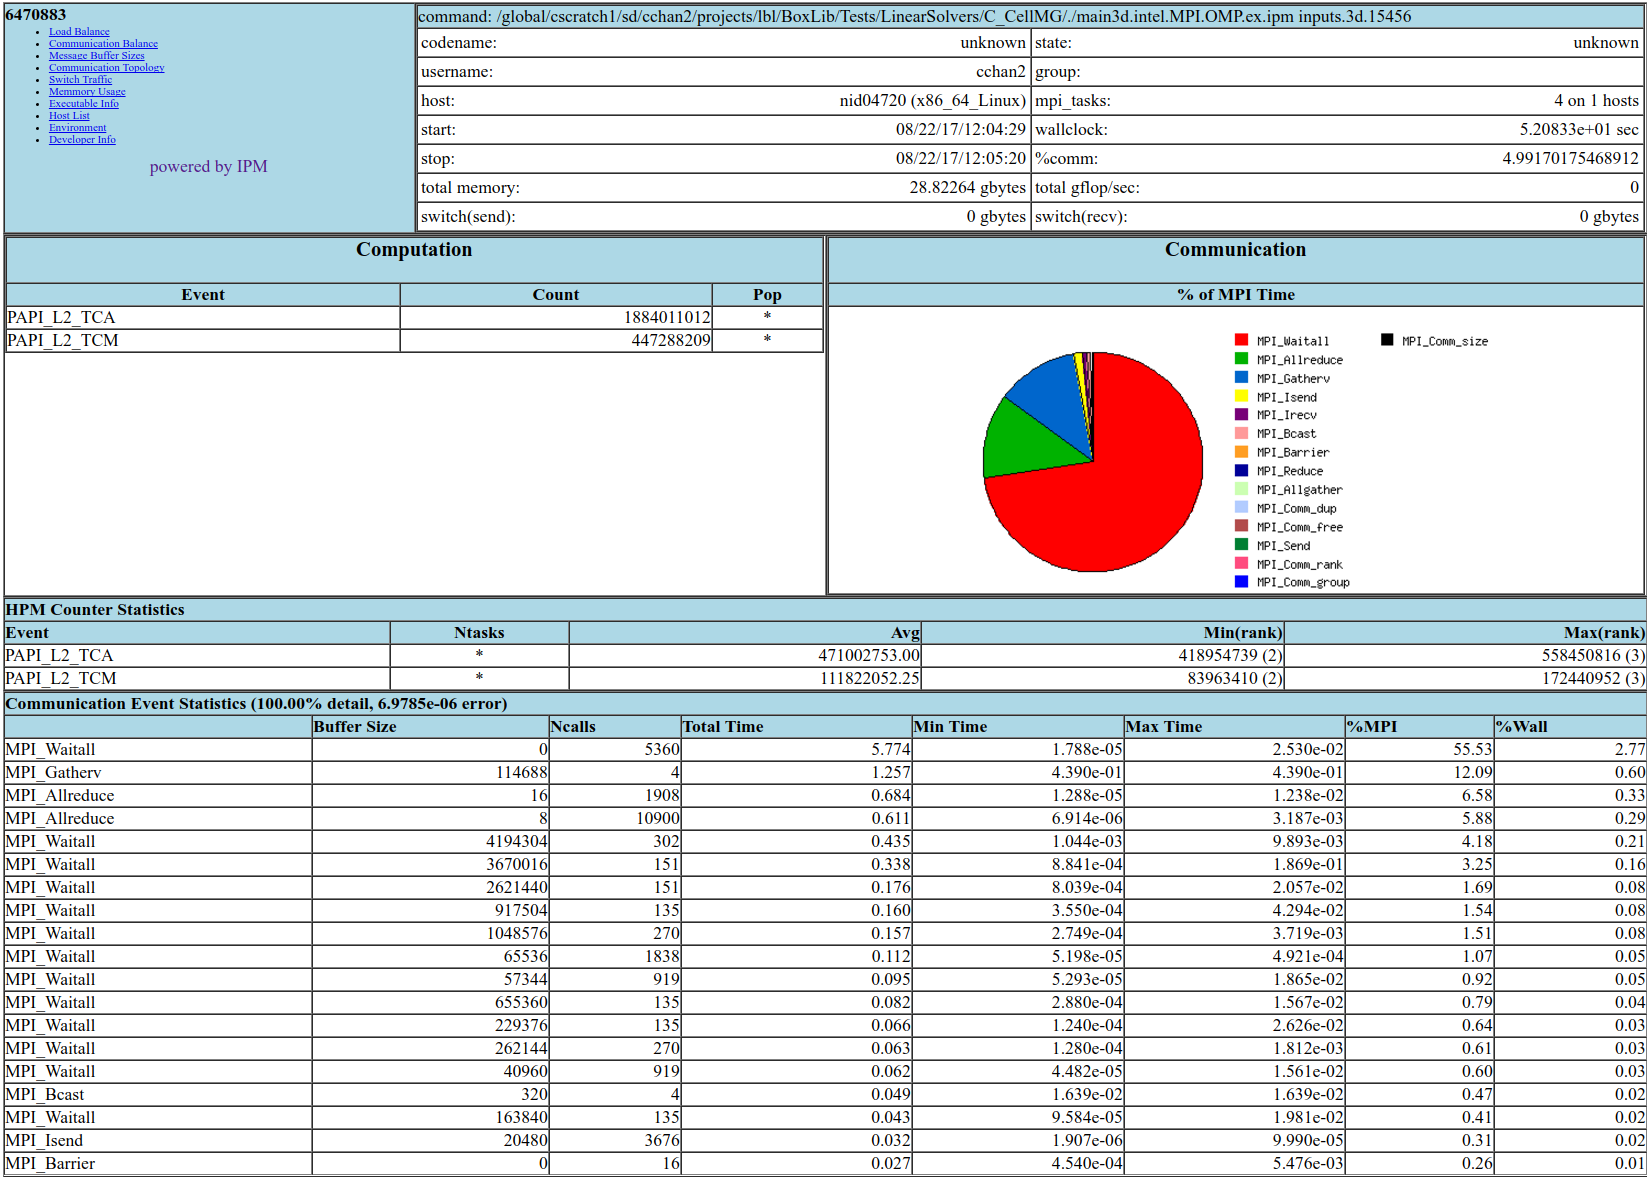
\includegraphics[width=\columnwidth]{Profiling/figs/summary.png}
  \end{center}
  \caption{
    Sample performance summary generated by IPM
  }
  \label{fig:ipm-summary}
\end{figure}

\begin{figure}
  \begin{center}
    \subfloat[Timings]{
      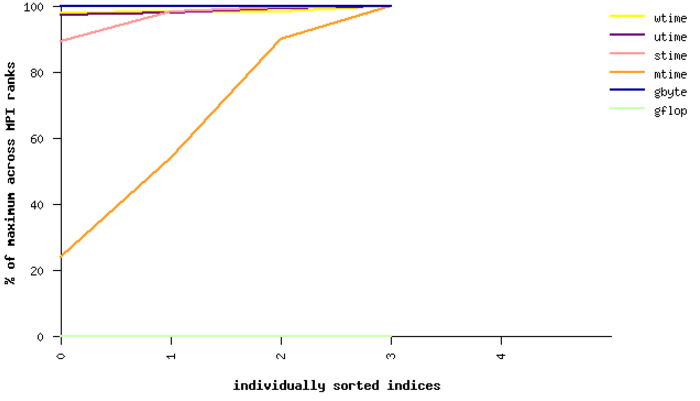
\includegraphics[width=0.49\columnwidth]{Profiling/figs/timings.png}
    }
    \subfloat[PAPI Counters]{
      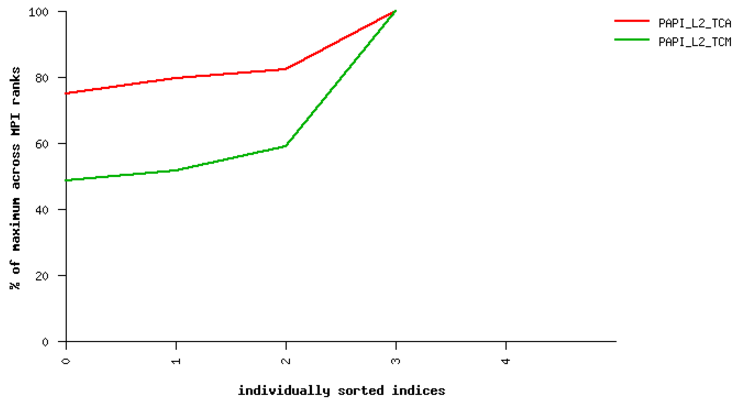
\includegraphics[width=0.49\columnwidth]{Profiling/figs/papi.png}
    } \\
    \subfloat[MPI Time by Function]{
      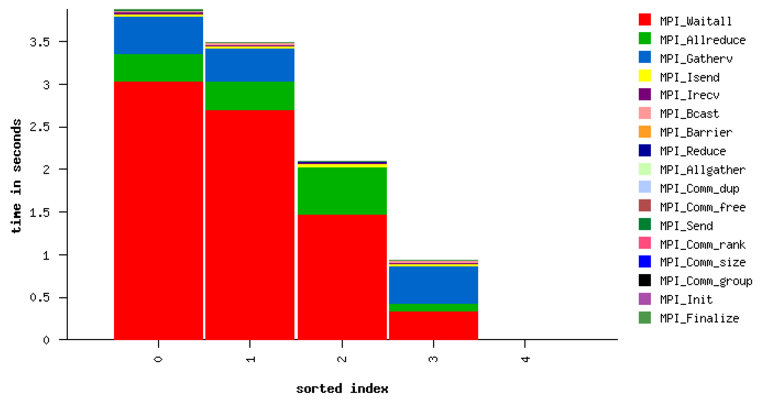
\includegraphics[width=0.49\columnwidth]{Profiling/figs/mpi.png}
    }
    \subfloat[MPI Time by Message Size]{
      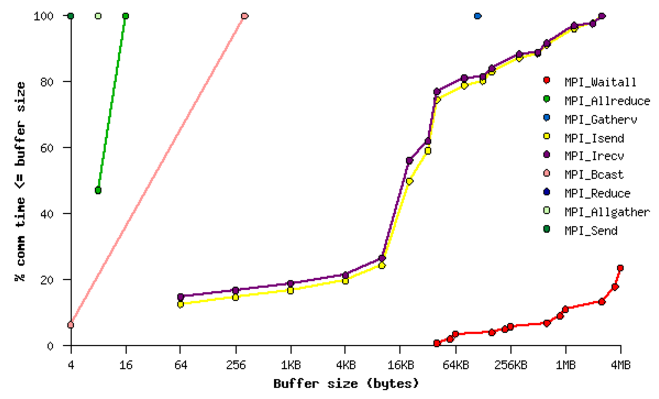
\includegraphics[width=0.49\columnwidth]{Profiling/figs/msgsizes.png}
    } \\
    \subfloat[Point-to-Point Communication Volume]{
      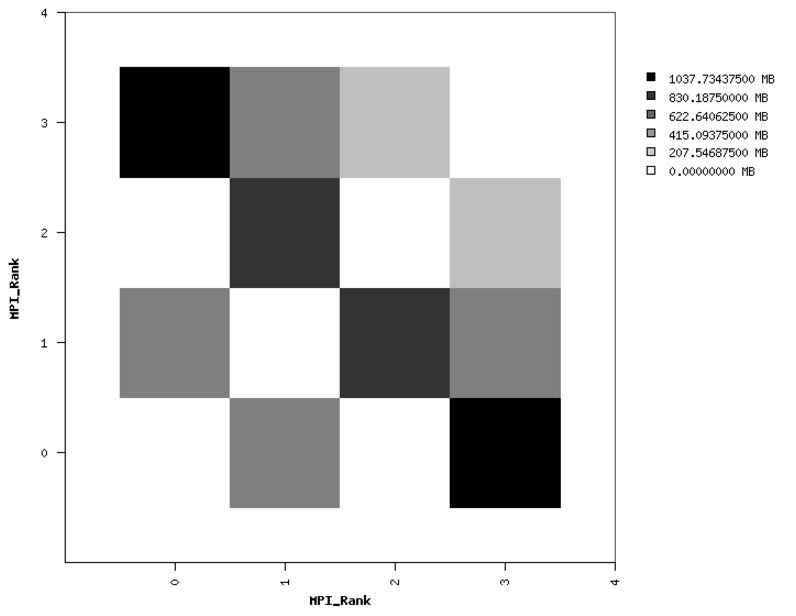
\includegraphics[width=0.49\columnwidth]{Profiling/figs/commtopo.png}
    }
  \end{center}
  \caption{
    Sample performance graphs generated by IPM
  }
  \label{fig:ipm-graphs}
\end{figure}
